% 附录 Q：等离子体诊断：从探针曲线到光谱（v1.14.0 新增）
% 数值唯一来源：tools/calc/appQ_calc.py -> tools/calc/appQ_calc.txt（正文与门禁的唯一来源）
% 时间单位写成 yr/day，避免中文字符进入数学字体；全部数字可用仓库脚本复算。
% 版权口径：只借鉴经典教材与文献的物理结论、公式形式与题型；文字、数值与表格自拟并独立复算。
% 离线环境无法核验 DOI，故只给书名、作者、年份、卷期页。

\section{诊断能测什么：先看手段与判据}
\label{sec:app-q-map}

前三章建立了模型，附录 M 到 P 把它用到加热、边界、推进与低温应用上。但模型对不对，取决于能不能
\textbf{测}。诊断（diagnostics）的共同困难是：等离子体内部不能直接伸手进去量，只能测"外部可观测
量"，再用一个已标定的模型反推内部参数。所以每一条诊断路线都由三件东西定义：\textbf{测什么原始量}、
\textbf{用什么模型反推}、\textbf{在什么条件下模型失效}。

\begin{table}[htbp]
  \centering
  \caption{五条常见诊断路线：原始量、反推参数与失效条件。失效条件一列的数字见本附录第 Q.2 至 Q.8 节。}
  \label{tab:app-q-map}
  \begin{tabular}{@{}p{2.6cm}p{3.2cm}p{4.4cm}p{5.2cm}@{}}
    \toprule
    手段 & 直接测量 & 反推的参数 & 失效条件（本附录给出判据） \\
    \midrule
    静电探针 & 探针电流 $I(V)$ & $T_e$、$n_e$、$V_p$、$V_f$、EEDF & 探针半径与 $\lambda_D$ 可比时收集理论不适用；鞘层有碰撞；射频干扰 \\
    磁探针（Rogowski、B-dot） & 线圈感应电压 $\propto \diff I/\diff t$ 或 $\diff B/\diff t$ & 放电电流、磁场 & 只能测变化量，不能测直流；积分时间常数不足 \\
    发射光谱（OES） & 谱线强度与谱线形状 & $T_e$（谱线比）、$T_i$（Doppler 宽度）、物种密度 & 谱线比要求日冕平衡；仪器宽度盖过 Doppler 宽度 \\
    汤姆孙散射 & 散射光光子数 & $n_e$、$T_e$、$T_i$（非相干散射） & 集体散射（Salpeter 参数不小）时谱形改用离子声波理论 \\
    微波干涉仪 & 相移 $\Delta\phi$ & 线积分密度 $\int n_e \diff l$ & 密度接近或超过截止密度 $n_c$ 时波不能传播 \\
    \bottomrule
  \end{tabular}
\end{table}

后文反复用到德拜长度，工程写法是把系数并成一个数：

\begin{equation}
  \lambda_D = 7433.9\sqrt{\frac{T_e[\mathrm{eV}]}{n_e[\mathrm{m^{-3}}]}}\ \mathrm{m},
  \qquad
  \lambda_D[\mathrm{\mu m}] = 7.4339\times10^{9}\sqrt{\frac{T_e[\mathrm{eV}]}{n_e[\mathrm{m^{-3}}]}}.
  \label{eq:app-q-debye}
\end{equation}

用附录 P 的五个工况代入，得到本附录的判据基准：刻蚀 $40.72\ \mathrm{\mu m}$、溅射与 PECVD
$105.13\ \mathrm{\mu m}$、医学射流 $2.88\ \mathrm{\mu m}$、大气压 DBD 微放电 $0.33\ \mathrm{\mu m}$、
聚变边界 $6.44\ \mathrm{\mu m}$。同一条公式跨五个量级——这就是为什么诊断手段必须按工况挑，
不能"买一台通用的"。

\textbf{出处：} Hutchinson《Principles of Plasma Diagnostics》第 2 版（诊断路线的总览与各章判据）；
Lieberman \& Lichtenberg《Principles of Plasma Discharges and Materials Processing》第 2 版第 6 章
（低温等离子体的探针诊断）；本书第 11 章鞘层与玻姆判据、附录 P 表 P.1。

\begin{figure}[htbp]
\centering
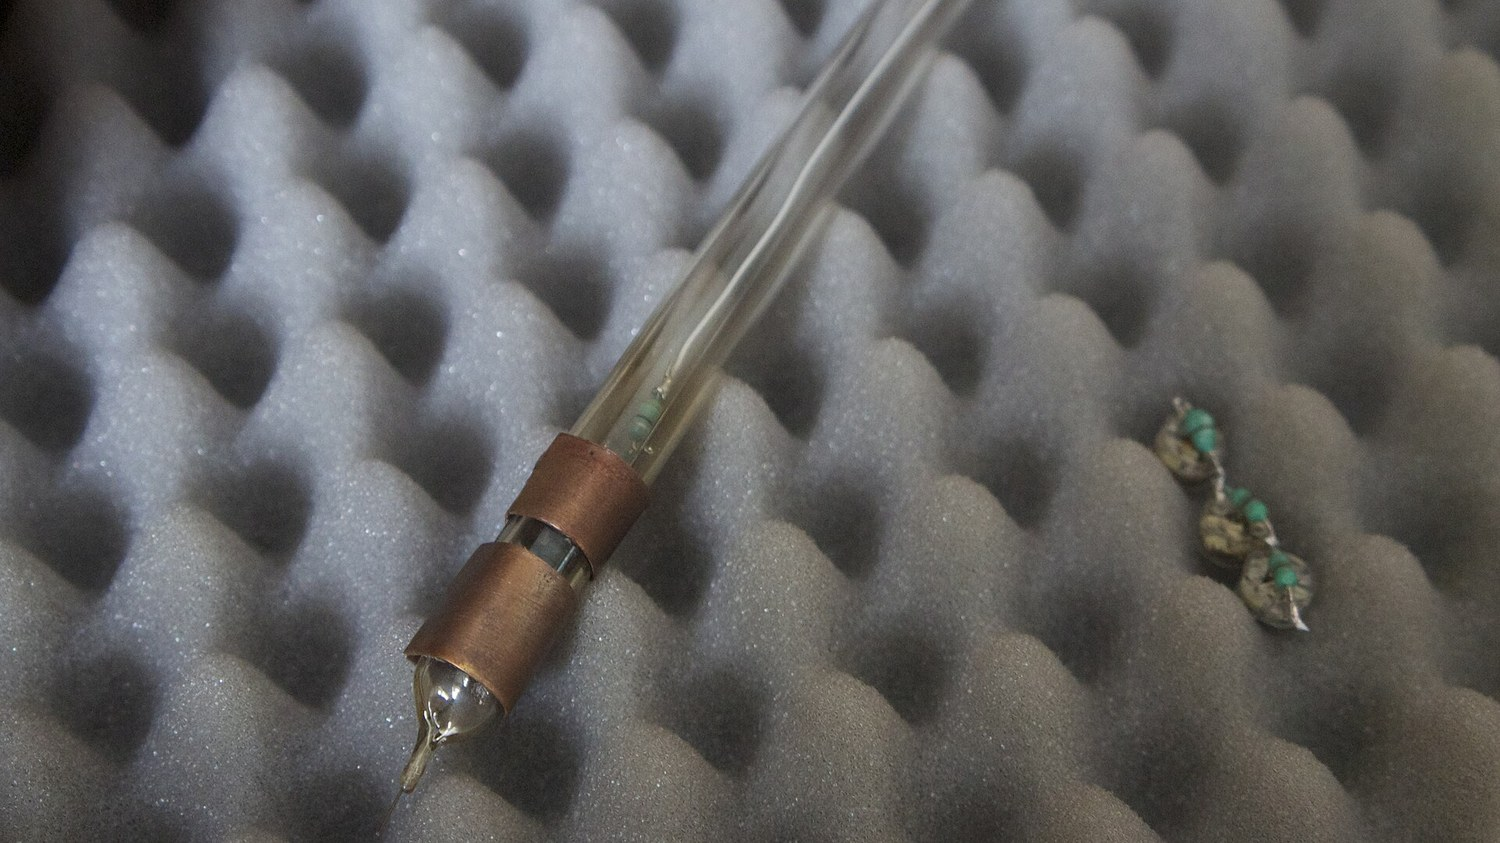
\includegraphics[width=0.78\textwidth]{../figures/q_rf_probe.jpg}
\caption{朗缪尔探针的实物：一根导线加一层鞘。本节把探针理论分成薄鞘与厚鞘两套，判据是探针半径与德拜长度之比；实物上它只是插进等离子体的一小段电极，难的是把射频干扰与二次发射挡在外面。}
\label{fig:photo-appq2}
\figsource{Vadmalis，CC BY-SA 3.0（Wikimedia Commons）}
\end{figure}

\section{静电探针：探针半径与德拜长度决定用哪套理论}
\label{sec:app-q-sheath}

探针插进等离子体后，周围必然形成鞘层，离子与电子的收集都被这个鞘层改写。因此第一件事不是读曲线，
而是判断\textbf{探针有多大、德拜长度有多长}：

\begin{equation}
  \frac{r_p}{\lambda_D} \ll 1 \;\Rightarrow\; \text{轨道运动限制（OML）},
  \qquad
  \frac{r_p}{\lambda_D} \gg 1 \;\Rightarrow\; \text{必须用径向运动（ABR）类理论}.
  \label{eq:app-q-oml}
\end{equation}

工程上常把 $r_p/\lambda_D\lesssim3$ 当作 OML 的可用边界、$\gtrsim20$ 必须换理论。取一支常见的
圆柱探针 $r_p=0.5\ \mathrm{mm}=500\ \mathrm{\mu m}$，在三种密度下算比值：

\begin{table}[htbp]
  \centering
  \caption{同一支 $r_p=0.5\ \mathrm{mm}$ 探针在三种密度下的适用性（$T_e=3\ \mathrm{eV}$，氩气）。}
  \label{tab:app-q-oml}
  \begin{tabular}{@{}rrrrl@{}}
    \toprule
    $n_e$ (m$^{-3}$) & $T_e$ (eV) & $\lambda_D$ ($\mu$m) & $r_p/\lambda_D$ & 可用理论 \\
    \midrule
    $1\times10^{17}$ & 3.0 & 40.72 & 12.28 & 超出 OML，需 ABR 类理论 \\
    $1\times10^{16}$ & 3.0 & 128.76 & 3.88 & 临界，需与 ABR 对照 \\
    $1\times10^{15}$ & 3.0 & 407.17 & 1.23 & OML 可用 \\
    \bottomrule
  \end{tabular}
\end{table}

结论很实用：在刻蚀工况（$10^{17}\ \mathrm{m^{-3}}$）下，要落回 OML 区需要 $r_p\le122.2\ \mathrm{\mu m}$，
比 $0.5\ \mathrm{mm}$ 细约 $4$ 倍；而同一支探针搬到 $10^{15}\ \mathrm{m^{-3}}$ 的余辉里就自洽了。
判据是\textbf{比值}，不是探针尺寸本身。

\textbf{出处：} Mott-Smith \& Langmuir, \emph{Physical Review} \textbf{28}, 727--763 (1926)（OML 收集
理论原始文献）；Hutchinson《Principles of Plasma Diagnostics》第 2 版探针各章（OML、ABR 与径向运动
理论的适用区间）；Lieberman \& Lichtenberg 第 2 版第 6 章。

\section{从 I--V 曲线读电子温度}
\label{sec:app-q-te}

单探针扫描电压得到 $I(V)$。在电子阻滞区（$V<V_p$）电子电流随电压指数上升，离子电流近似为常数：

\begin{equation}
  I(V) = I_{es0}\exp\!\left(\frac{V-V_p}{T_e}\right) - I_{is},
  \label{eq:app-q-iv}
\end{equation}

于是对数斜率直接给出电子温度：

\begin{equation}
  \frac{\diff(\ln I_e)}{\diff V} = \frac{1}{T_e}
  \qquad\Longleftrightarrow\qquad
  T_e[\mathrm{eV}] = \left[\frac{\diff(\ln I_e)}{\diff V}\right]^{-1}.
  \label{eq:app-q-slope}
\end{equation}

取一组合成数据（$T_e=3.0\ \mathrm{eV}$、$I_{es0}=10\ \mathrm{mA}$、$I_{is}=1\ \mathrm{mA}$）：

\begin{table}[htbp]
  \centering
  \caption{合成单探针曲线：电子电流与净电流（$I_{es0}=10\ \mathrm{mA}$，$T_e=3.0\ \mathrm{eV}$）。}
  \label{tab:app-q-iv}
  \begin{tabular}{@{}rrr@{}}
    \toprule
    $V-V_p$ (V) & $I_e$ (mA) & $I_{\mathrm{net}}$ (mA) \\
    \midrule
    0.0 & 10.0000 & 9.0000 \\
    $-1.0$ & 7.1653 & 6.1653 \\
    $-2.0$ & 5.1342 & 4.1342 \\
    $-3.0$ & 3.6788 & 2.6788 \\
    $-4.0$ & 2.6360 & 1.6360 \\
    $-6.0$ & 1.3534 & 0.3534 \\
    $-8.0$ & 0.6948 & $-0.3052$ \\
    \bottomrule
  \end{tabular}
\end{table}

取 $V-V_p=-3\ \mathrm{V}$ 与 $-6\ \mathrm{V}$ 两点做对数斜率，两种做法差一倍：

\begin{itemize}
  \item \textbf{先减离子电流}（正确）：$\diff(\ln I_e)/\diff V = 0.333333\ \mathrm{V^{-1}}$
        $\Rightarrow T_e=3.0000\ \mathrm{eV}$；
  \item \textbf{直接对净电流取对数}（常见错误）：斜率变成 $0.675218\ \mathrm{V^{-1}}$
        $\Rightarrow T_e=1.4810\ \mathrm{eV}$，\textbf{低估 $50.63\%$}。
\end{itemize}

错误的大小取决于离子电流占净电流的比例，所以\textbf{选点越靠近 $V_p$、漏减造成的偏差越小}：
同样不减 $I_{is}$，改用 $-1\ \mathrm{V}$ 与 $-2\ \mathrm{V}$ 两点，得到 $T_e=2.5022\ \mathrm{eV}$，
只低估 $16.59\%$。实际操作中还要避开电子饱和区，落到"离子电流可忽略、又没进饱和"的中间段。

\textbf{出处：} Druyvesteyn, \emph{Zeitschrift f\"ur Physik} \textbf{64}, 781--798 (1930)（由探针曲线
二次导数求电子能量分布）；Godyak \& Demidov, \emph{Journal of Physics D} \textbf{44}, 233001 (2011)
（探针测 EEDF 的可靠性与误差来源综述）；Lieberman \& Lichtenberg 第 2 版第 6 章。

\section{从离子饱和电流读密度}
\label{sec:app-q-ne}

偏压远低于 $V_f$ 时只剩离子电流，它在鞘层扩张后近似写成

\begin{equation}
  I_{is} = 0.6\,e\,n_e\,c_s\,A_p,
  \qquad
  c_s = \sqrt{\frac{k_BT_e}{m_i}},
  \label{eq:app-q-iis}
\end{equation}

其中 $0.6$ 是圆柱探针鞘层扩张的经验因子（把裸玻姆通量 $e n_e c_s$ 修正到实际收集面）。
取 $r_p=0.5\ \mathrm{mm}$、$l_p=10\ \mathrm{mm}$，则 $A_p=2\pi r_p l_p=3.141593\times10^{-5}\ \mathrm{m^2}$；
$T_e=3.0\ \mathrm{eV}$ 的氩离子玻姆速度 $c_s=2691.81\ \mathrm{m/s}$，于是

\begin{equation}
  j_i = e n_e c_s = 43.1275\ \mathrm{A/m^2} = 4.3127\ \mathrm{mA/cm^2},
  \label{eq:app-q-ji}
\end{equation}

与附录 P 表 P.1 的刻蚀基准 $4.313\ \mathrm{mA/cm^2}$ 完全一致——\textbf{两条独立路径必须给出同一个数}，
这就是自检。$A_p$ 上的离子饱和电流是 $1.354890\ \mathrm{mA}$（裸玻姆）或 $0.812934\ \mathrm{mA}$
（含 $0.6$ 因子）。若实测 $I_{is}=1.000\ \mathrm{mA}$，反推

\begin{equation}
  n_e = \frac{I_{is}}{0.6\,e\,c_s\,A_p} = 1.2301\times10^{17}\ \mathrm{m^{-3}};
  \label{eq:app-q-ne}
\end{equation}

漏掉 $0.6$ 因子会得到 $7.3807\times10^{16}\ \mathrm{m^{-3}}$，\textbf{低估 $40.0\%$}。
误差传递同样简单（各项独立相加）：

\begin{equation}
  \frac{\delta n_e}{n_e} = \frac{\delta I_{is}}{I_{is}} + \frac{\delta A_p}{A_p} + \frac12\frac{\delta T_e}{T_e}.
  \label{eq:app-q-err}
\end{equation}

指数 $1/2$ 来自 $c_s\propto\sqrt{T_e}$：\textbf{$T_e$ 的 $10\%$ 误差只带来 $5\%$ 的密度误差}，
而探针面积错了 $5\%$ 就直接错 $5\%$。所以探针诊断里最该盯住的不是电子温度，而是\textbf{有效收集面积}
（边缘效应、薄膜沉积、探针杆暴露）。

\textbf{出处：} Lieberman \& Lichtenberg 第 2 版第 6 章（离子饱和电流与 $0.6$ 因子）；Hutchinson
《Principles of Plasma Diagnostics》第 2 版探针各章（面积效应与二次电子）；本书附录 P 表 P.1 与
式 \eqref{eq:app-p-flux}。

\section{悬浮电位与等离子体电位}
\label{sec:app-q-float}

不放任何偏压时，探针（或任何绝缘表面）自动停在电子电流与离子电流相等处。用随机通量电子
$\frac14 n_ev_e$ 对玻姆离子 $n_ec_s$：

\begin{equation}
  V_p - V_f = T_e\ln\frac{\bar v_e}{4c_s},
  \qquad
  \bar v_e = \sqrt{\frac{8k_BT_e}{\pi m_e}}.
  \label{eq:app-q-float}
\end{equation}

$T_e=3.0\ \mathrm{eV}$ 时 $\bar v_e=1.1592\times10^{6}\ \mathrm{m/s}$，比值 $\bar v_e/(4c_s)=107.6559$，
故 $V_p-V_f=4.6789\,T_e=14.0368\ \mathrm{V}$——系数 $4.6789$ 与附录 P 的 $e\phi_f/k_BT_e=4.6789$
逐位一致。若离子电流那一侧改用含 $0.6$ 因子的式 \eqref{eq:app-q-iis}，比值变成 $179.4264$，
得到 $5.1898\,T_e=15.5693\ \mathrm{V}$。两式之差是定值：

\begin{equation}
  \Delta(V_p-V_f) = T_e\ln\frac{1}{0.6} = 1.5325\ \mathrm{V}\quad(T_e=3\ \mathrm{eV}).
  \label{eq:app-q-floatdiff}
\end{equation}

这不是算错，而是\textbf{收集模型不同}。

做量级自检时若发现自己的悬浮电位和教科书差 $T_e\ln(1/0.6)$，先检查用的是哪一套离子电流公式，再怀疑算错。

\textbf{出处：} Hutchinson《Principles of Plasma Diagnostics》第 2 版探针各章（悬浮电位与
浮动表面）；Lieberman \& Lichtenberg 第 2 版第 6 章；本书第 11 章玻姆判据、附录 P 式
\eqref{eq:app-p-noneq} 附近的非平衡讨论。

\section{磁诊断：Rogowski 线圈与 RC 积分}
\label{sec:app-q-magnetic}

磁探针不接触等离子体，代价是只能测\textbf{变化量}。环形 Rogowski 线圈套住放电电流，
互感由几何决定：

\begin{equation}
  M = \frac{\mu_0 N A_c}{2\pi r_{\mathrm{mean}}},
  \qquad
  V_{\mathrm{coil}} = M\frac{\diff I}{\diff t}.
  \label{eq:app-q-mutual}
\end{equation}

取 $N=1000$ 匝、单匝面积 $A_c=1\ \mathrm{cm^2}$、平均半径 $r_{\mathrm{mean}}=5\ \mathrm{cm}$，
得 $M=4.0000\times10^{-7}\ \mathrm{H}=400.0\ \mathrm{nH}$。若放电电流 $100\ \mathrm{A}$ 在
$1\ \mathrm{\mu s}$ 内上升，$\diff I/\diff t=1.000\times10^{8}\ \mathrm{A/s}$，线圈直接输出
$40.00\ \mathrm{V}$——太高，且波形是 $\diff I/\diff t$ 而不是 $I$，所以必须积分。用最简单的
RC 积分器：

\begin{equation}
  V_{\mathrm{out}} = \frac{MI}{RC},
  \qquad
  S = \frac{M}{RC},
  \label{eq:app-q-rc}
\end{equation}

要求 $RC\gg$ 脉宽。取 $R=50\ \Omega$、$C=1.0\ \mathrm{\mu F}$，$RC=50.0\ \mathrm{\mu s}$
是脉宽的 $50$ 倍，于是 $V_{\mathrm{out}}=0.8000\ \mathrm{V}$，灵敏度
$S=8.0000\times10^{-3}\ \mathrm{V/A}$。反向校验：$V_{\mathrm{coil}}\times$ 脉宽 $/RC
=40.00\times(1/50)=0.8000\ \mathrm{V}$，两条路径一致。

设计上的两难写在这里：$RC$ 太小则积分不成立（输出退化成 $\diff I/\diff t$），$RC$ 太大则灵敏度
$S$ 变小（$1\ \mathrm{A}$ 只给 $8\ \mathrm{mV}$，需要低噪声放大）。B-dot 探针同理，只是把它测的
$\diff B/\diff t$ 换成磁场。

\textbf{出处：} Hutchinson《Principles of Plasma Diagnostics》第 2 版磁诊断各章（Rogowski 线圈、
磁探针与积分器设计）；本书第 12 章磁探针与放电电流测量的相关小节。

\section{光学诊断：Doppler 宽度与谱线比}
\label{sec:app-q-optical}

光学诊断的优点是完全不扰动等离子体，缺点是只能看\textbf{视线积分}。两条最常用的路线：

\textbf{（1）谱线宽度给离子温度。}热运动造成 Doppler 增宽，半高全宽为

\begin{equation}
  \Delta\lambda_{\mathrm{FWHM}} = 7.16\times10^{-7}\,\lambda\sqrt{\frac{T_i[\mathrm{K}]}{M[\mathrm{amu}]}},
  \label{eq:app-q-doppler}
\end{equation}

对 Ar I $696.5\ \mathrm{nm}$：室温 $300\ \mathrm{K}$ 给出 $1.3666\ \mathrm{pm}$，$T_i=0.5\ \mathrm{eV}$
给出 $6.0101\ \mathrm{pm}$，$T_i=3\ \mathrm{eV}$ 给出 $14.7218\ \mathrm{pm}$。普通光谱仪的仪器宽度约
$50\ \mathrm{pm}$（$0.05\ \mathrm{nm}$），是室温 Doppler 宽度的 $37$ 倍——\textbf{低分辨率光谱仪
根本测不出离子温度}，必须用高分辨光栅或法布里--珀罗标准具。

\textbf{（2）谱线强度比给电子温度。}日冕平衡下，两条同种离子的谱线强度比只通过阈值能差依赖 $T_e$：

\begin{equation}
  \frac{I_1}{I_2} = K\exp\!\left(-\frac{\Delta E}{T_e}\right),
  \qquad
  K \equiv \frac{A_1g_1\lambda_2}{A_2g_2\lambda_1},
  \label{eq:app-q-oes}
\end{equation}

氩的 $750.4\ \mathrm{nm}$ 与 $811.5\ \mathrm{nm}$ 这一对阈值能差约 $0.40\ \mathrm{eV}$。把 $K$ 归一到
$1$ 只看敏感性：

\begin{table}[htbp]
  \centering
  \caption{双线强度比到电子温度（$\Delta E=0.40\ \mathrm{eV}$，$K=1$）。}
  \label{tab:app-q-oes}
  \begin{tabular}{@{}rr@{}}
    \toprule
    强度比 $I_1/I_2$ & $T_e$ (eV) \\
    \midrule
    0.950 & 7.7983 \\
    0.900 & 3.7965 \\
    0.875 & 2.9956 \\
    0.850 & 2.4613 \\
    0.750 & 1.3904 \\
    0.500 & 0.5771 \\
    \bottomrule
  \end{tabular}
\end{table}

指数关系意味着\textbf{误差被放大}：强度比从 $0.875$ 变到 $0.850$ 或 $0.900$（$\pm2.9\%$），
$T_e$ 就从 $2.9956\ \mathrm{eV}$ 变成 $2.4613$ 或 $3.7965\ \mathrm{eV}$（$-17.8\%$ 与 $+26.7\%$），
放大约 $10$ 倍。而"把 $K$ 当成 $1$"本身就是简化：严格的 $K$ 要查 $A_{ji}$、$g_j$，还要考虑级联
与自吸收，所以这一路线的定位是\textbf{快速量级监测}，不是精密测温。绝对强度还能反推探测极限：
$1\ \mathrm{mW}$ 的 $750\ \mathrm{nm}$ 光进入 $1\%$ 通量的光谱仪是 $3.7756\times10^{13}$ 光子/s，
曝光 $1\ \mathrm{ms}$ 得 $3.776\times10^{10}$ 个光子——探测器会饱和，实际必须衰减或缩短曝光。

\textbf{出处：} Fantz, \emph{Plasma Sources Science and Technology} \textbf{15}, S137--S147 (2006)
（等离子体光谱基础与谱线比方法）；Hutchinson《Principles of Plasma Diagnostics》第 2 版发射光谱
各章（Doppler 增宽与仪器宽度）。

\section{汤姆孙散射与微波干涉仪}
\label{sec:app-q-scatter}

\textbf{（1）汤姆孙散射}直接测电子，不依赖平衡假设。散射谱的形状由一个无量纲数决定：散射参数
$\alpha=1/(k\lambda_D)$，其中散射波矢 $k=2k_i\sin(\theta/2)$。

\begin{equation}
  \alpha = \frac{1}{k\lambda_D} \ll 1:\ \text{非相干（电子特征）},
  \qquad
  \alpha \gg 1:\ \text{集体散射（出现离子声波特征）}.
  \label{eq:app-q-salpeter}
\end{equation}

入射 $532\ \mathrm{nm}$、散射角 $90^\circ$ 时 $k=1.6703\times10^{7}\ \mathrm{m^{-1}}$：

\begin{table}[htbp]
  \centering
  \caption{三个工况的 Salpeter 参数（$532\ \mathrm{nm}$、$90^\circ$）。}
  \label{tab:app-q-salpeter}
  \begin{tabular}{@{}lrrr@{}}
    \toprule
    工况 & $\lambda_D$ (m) & $k\lambda_D$ & $\alpha=1/(k\lambda_D)$ \\
    \midrule
    刻蚀 & $4.0717\times10^{-5}$ & 680.08 & $1.4704\times10^{-3}$ \\
    大气压 DBD & $3.3246\times10^{-7}$ & 5.55 & $1.8009\times10^{-1}$ \\
    聚变边界 & $6.4380\times10^{-6}$ & 107.53 & $9.2997\times10^{-3}$ \\
    \bottomrule
  \end{tabular}
\end{table}

三行都落在非相干区（$\alpha\ll1$），所以都能按"每个电子独立散射"处理。可测性用光子账算：

\begin{equation}
  N_s = n_e L\,\sigma_T\,\Delta\Omega\,N_{\mathrm{ph}},
  \qquad
  \sigma_T = 6.6525\times10^{-29}\ \mathrm{m^2},
  \label{eq:app-q-photons}
\end{equation}

$1\ \mathrm{J}$、$10\ \mathrm{ns}$ 的 $532\ \mathrm{nm}$ 激光是 $2.6782\times10^{18}$ 个光子，
照到 $n_e=10^{17}\ \mathrm{m^{-3}}$、$L=10\ \mathrm{mm}$、收集立体角 $0.01\ \mathrm{sr}$ 上，
每发只收到 $1781.6$ 个散射光子，统计误差 $2.37\%$——\textbf{单发就能测，但余量不大}。

\textbf{（2）微波干涉仪}测的是相移，与密度成正比：

\begin{equation}
  \Delta\phi = \frac{\omega}{c}\cdot\frac{n_e}{2n_c}\cdot L,
  \qquad
  n_c = \frac{\epsilon_0m_e\omega^2}{e^2} = 1.2404\times10^{18}\ \mathrm{m^{-3}}\ \text{（10 GHz）}.
  \label{eq:app-q-microwave}
\end{equation}

$n_e=10^{17}\ \mathrm{m^{-3}}$、$L=0.3\ \mathrm{m}$ 时 $n_e/n_c=0.080616$，
$\Delta\phi=2.5344\ \mathrm{rad}=0.4034$ 条纹——相位法测到不到半条条纹，说明这条路线适合
\textbf{更高密度}。频率的选择由密度上限决定：要测附录 P 里医学射流的
$10^{19}\ \mathrm{m^{-3}}$，必须 $f>28.39\ \mathrm{GHz}$。反过来，$10\ \mathrm{GHz}$ 的
$n_c=1.2404\times10^{18}\ \mathrm{m^{-3}}$ 也正是刻蚀等离子体的适用上限。

\textbf{出处：} Sheffield, Froula, Glenzer \& Luhmann《Plasma Scattering of Electromagnetic
Radiation》第 2 版（汤姆孙散射谱与 Salpeter 参数）；Heald \& Wharton《Plasma Diagnostics with
Microwaves》（微波干涉法、截止密度）；Hutchinson《Principles of Plasma Diagnostics》第 2 版
散射与折射率各章。

\section{误差与自检：把不确定度写成结论}
\label{sec:app-q-error}

测量报告的最后一句话必须是"我测到多少，误差多大，为什么"。把本附录用到的传递关系集中起来：

\begin{table}[htbp]
  \centering
  \caption{被测量的相对误差如何传到最后结论（本附录各节的系数）。}
  \label{tab:app-q-error}
  \begin{tabular}{@{}p{3.4cm}p{7.0cm}r@{}}
    \toprule
    被测量 & 主要来源 & 传递指数 \\
    \midrule
    $I_{is}$ & 读数、射频补偿、二次电子 & 1 \\
    $A_p$ & 边缘效应、薄膜沉积、探针杆暴露 & 1 \\
    $T_e$ & 选点区间、漏减 $I_{is}$、非麦氏尾部 & $1/2$（进 $n_e$） \\
    谱线强度比 & 标定、自吸收、级联 & 放大约 10 倍（进 $T_e$） \\
    散射光子数 $N_s$ & 散粒噪声、杂散光 & $1/\sqrt{N_s}$ \\
    \bottomrule
  \end{tabular}
\end{table}

系统误差永远比统计误差更危险，因为它们\textbf{不随平均次数下降}。低温等离子体探针诊断里有四个
固定嫌疑：射频干扰（需要 RF 补偿探针）、二次电子发射（污染离子电流）、探针表面的绝缘膜与沉积
（改变有效面积）、以及参考电极面积不足（"等离子体电位"其实在漂）。这四条都不需要新公式，只需要
\textbf{换一种独立手段交叉验证}——探针给的 $n_e$ 用微波干涉仪复核，OES 给的 $T_e$ 用探针复核，
对不上就先怀疑系统误差。

\begin{tip}{先问能不能测到，再问测得多准}{tip-appq-limit}
本节六节诊断路线都可以用一句话否决：\textbf{把"能测到的最小信号"和"可用的模型区间"算出来}。
探针要算 $r_p/\lambda_D$ 与 $I_{is}$ 是否大于噪声；光谱要算 Doppler 宽度是否大于仪器宽度；
汤姆孙散射要算每发收到几个光子；微波要算 $n_e/n_c$ 是否接近 $1$。这四步都只用乘除，却能在买设备
之前就把不合适的方案筛掉。
\end{tip}

\textbf{出处：} Godyak \& Demidov, \emph{Journal of Physics D} \textbf{44}, 233001 (2011)（探针诊断的
系统误差清单与可靠性判据）；Hutchinson《Principles of Plasma Diagnostics》第 2 版各章的误差讨论；
本书附录 I「测量与不确定度」一节（学习方法侧的同一套口径）。

\section{六道估算练习}
\label{sec:app-q-problems}


\textbf{练习 1（两点法读 $T_e$）}。某单探针曲线：$I_{es0}=5.0\ \mathrm{mA}$、
$I_{is}=0.5\ \mathrm{mA}$，在 $V-V_p=-2\ \mathrm{V}$ 与 $-4\ \mathrm{V}$ 处测得净电流
$I_{\mathrm{net}}=1.3394\ \mathrm{mA}$ 与 $0.1767\ \mathrm{mA}$。(1) 先减 $I_{is}$ 再取对数斜率求 $T_e$；
(2) 若直接对净电流取斜率，得到多少？说明偏差方向。

\textbf{解答}：先减 $I_{is}$ 得 $I_e=1.8394$ 与 $0.6767\ \mathrm{mA}$，斜率
$(\ln1.8394-\ln0.6767)/2=0.5\ \mathrm{V^{-1}}$，故 $T_e=2.0000\ \mathrm{eV}$。直接取净电流斜率得
$1.0127\ \mathrm{V^{-1}}$，$T_e=0.9873\ \mathrm{eV}$，\textbf{低估 $50.6\%$}——离子电流在小信号处
占比更大。

\textbf{练习 2（离子饱和电流反推密度）}。圆柱探针 $r_p=0.4\ \mathrm{mm}$、$l_p=8.0\ \mathrm{mm}$，
氩气 $T_e=2.5\ \mathrm{eV}$，实测 $I_{is}=0.60\ \mathrm{mA}$。求 $n_e$（用式 \eqref{eq:app-q-iis}）。

\textbf{解答}：$A_p=2.010619\times10^{-5}\ \mathrm{m^2}$，$c_s=2457.27\ \mathrm{m/s}$，
$n_e=I_{is}/(0.6ec_sA_p)=1.2633\times10^{17}\ \mathrm{m^{-3}}$。

\textbf{练习 3（判据选理论）}。$n_e=5\times10^{16}\ \mathrm{m^{-3}}$、$T_e=4.0\ \mathrm{eV}$，
探针半径 $1\ \mathrm{mm}$。(1) 求 $\lambda_D$ 与 $r_p/\lambda_D$；(2) 若要回到 OML 适用区
（取边界 $3$），探针最粗能到多少？

\textbf{解答}：$\lambda_D=6.6491\times10^{-5}\ \mathrm{m}=66.49\ \mathrm{\mu m}$，
$r_p/\lambda_D=15.04$，超出 OML 区，需 ABR 类理论。要 $r_p\le3\lambda_D=199.5\ \mathrm{\mu m}$，
即换成直径 $0.4\ \mathrm{mm}$ 以下的细丝。

\textbf{练习 4（Rogowski 线圈设计）}。$N=500$ 匝、$A_c=2\ \mathrm{cm^2}$、
$r_{\mathrm{mean}}=4\ \mathrm{cm}$，测 $200\ \mathrm{A}$、$2\ \mathrm{\mu s}$ 上升的放电。
(1) 求互感与线圈原始输出电压；(2) 取 $R=100\ \Omega$、$C=1.0\ \mathrm{\mu F}$，求积分输出与灵敏度。

\textbf{解答}：$M=5.0000\times10^{-7}\ \mathrm{H}=500\ \mathrm{nH}$；
$V_{\mathrm{coil}}=MI/t_{\mathrm{rise}}=50.00\ \mathrm{V}$；
$RC=100\ \mathrm{\mu s}$，$V_{\mathrm{out}}=MI/(RC)=1.0000\ \mathrm{V}$，
$S=5.0000\times10^{-3}\ \mathrm{V/A}$。

\textbf{练习 5（汤姆孙散射可测性）}。激光 $0.5\ \mathrm{J}$、$532\ \mathrm{nm}$、
$n_e=5\times10^{18}\ \mathrm{m^{-3}}$、$L=1\ \mathrm{cm}$、收集立体角 $0.02\ \mathrm{sr}$。
求每发散射光子数与统计误差。

\textbf{解答}：$N_{\mathrm{ph}}=1.33895\times10^{18}$（每个光子 $3.7339\times10^{-19}\ \mathrm{J}$），
$N_s=n_eL\sigma_T\Delta\Omega N_{\mathrm{ph}}=89081$ 个，统计误差
$1/\sqrt{N_s}=0.335\%$。

\textbf{练习 6（微波干涉仪选频）}。要测 $n_e=3\times10^{18}\ \mathrm{m^{-3}}$：(1) 最低工作频率是多少？
(2) 取 $20\ \mathrm{GHz}$、$L=0.2\ \mathrm{m}$，求相移（rad 与条纹数）。

\textbf{解答}：$f>15.55\ \mathrm{GHz}$。$20\ \mathrm{GHz}$ 时
$n_c=4.9618\times10^{18}\ \mathrm{m^{-3}}$，$n_e/n_c=0.6046$，
$\Delta\phi=25.3439\ \mathrm{rad}=4.0336$ 条纹——这一次条纹足够多，相位法可行。

\begin{tip}{下一步读什么}{tip-appq-next}
诊断是把前面所有章节"变成可验证"的一环。建议按三条线继续：\textbf{（1）模型侧}回到第 11 章鞘层与
玻姆判据、附录 K.3 与 K.7（鞘层加速与 Child--Langmuir 律），因为探针曲线的一半信息都在鞘层里；
\textbf{（2）误差侧}读附录 I「测量与不确定度」，把误差写成物理结论而不是小数点位数；
\textbf{（3）应用侧}回到附录 P，用那里的五个工况当练习背景——同一个诊断在五个量级上能否用，
正是本附录练习 3 与练习 6 想训练的判断。
\end{tip}

\section{来源、分级与版权说明}
\label{sec:app-q-source}

本附录只借鉴经典教材与文献的\textbf{物理结论、公式形式与题型}，全部文字、数值与表格由本书自拟并
用 \texttt{appQ\_calc.py} 独立复算。离线环境无法核验 DOI，故只给可核对的定位信息。

\begin{table}[htbp]
  \centering
  \caption{本附录借鉴的来源与借用内容。}
  \label{tab:app-q-source}
  \begin{tabular}{@{}p{4.8cm}p{5.6cm}p{5.0cm}@{}}
    \toprule
    来源 & 定位 & 本附录借用的内容 \\
    \midrule
    Hutchinson《Principles of Plasma Diagnostics》 & 第 2 版，Cambridge University Press (2002) & 诊断路线总览、探针收集理论区间、磁诊断与积分器、光谱与散射各章判据 \\
    Lieberman \& Lichtenberg《Principles of Plasma Discharges and Materials Processing》 & 第 2 版第 6 章，Wiley (2005) & 离子饱和电流与 $0.6$ 鞘层扩张因子、悬浮电位 \\
    Mott-Smith \& Langmuir & \emph{Physical Review} \textbf{28}, 727--763 (1926) & OML 收集理论的原始表述 \\
    Druyvesteyn & \emph{Zeitschrift f\"ur Physik} \textbf{64}, 781--798 (1930) & 由探针曲线二次导数求电子能量分布 \\
    Godyak \& Demidov & \emph{Journal of Physics D} \textbf{44}, 233001 (2011) & 探针诊断的系统误差清单与可靠性判据 \\
    Fantz & \emph{Plasma Sources Science and Technology} \textbf{15}, S137--S147 (2006) & 发射光谱基础、谱线比与 Doppler 增宽 \\
    Sheffield, Froula, Glenzer \& Luhmann & 第 2 版，Academic Press (2011) & 汤姆孙散射谱与 Salpeter 参数 \\
    Heald \& Wharton《Plasma Diagnostics with Microwaves》 & Wiley (1965) & 微波干涉法、截止密度与相移公式 \\
    Chen《Introduction to Plasma Physics and Controlled Fusion》 & 第 3 版，Springer (2016) & 德拜长度与玻姆速度的教学口径 \\
    Langmuir & \emph{Physical Review} \textbf{2}, 450--486 (1913) & 空间电荷限制电流（与 Child 1911 配对，见附录 K.7） \\
    \bottomrule
  \end{tabular}
\end{table}

\begin{itemize}
  \item 本附录\textbf{不复制}任何教材或论文的题目、解答、图表与数据表；表格中的参数与判据区间属于
        教科书公共知识，文字表述与全部数值由本书自拟并独立复算；
  \item 所有数值均可用仓库脚本 \texttt{appQ\_calc.py} 复算，与正文、门禁三方一致；
  \item 诊断手段的取舍属于工程判断，本附录给出的是\textbf{量级判据}，实际装置还需考虑成本、
        空间与安全性。
\end{itemize}
